\documentclass{article}
\usepackage[utf8]{inputenc}

\title{Hw1 Report}
\author{Muhammed Yasir Fidan }
\date{March 2021}

\usepackage{natbib}
\usepackage{graphicx}

\begin{document}

\maketitle

\section{Report}
\textbf{Compile and Run} \\
\\
Firstly I compile my program with gcc -o myFind hw1.c -std=c99 -Wall -D\_BSD\_SOURCE -D\_POSIX\_C\_SOURCE in makefile, so there is no warning when using -Wall command. Then I run my program with Valdring for checking there is memory leak or not and there is no any memory leak.\\
\\
\textbf{Taking arguments} \\
\\
I used getotp for getting arguments, also I hold booleans for all arguments so I can check which arguments enter or not. For example if user enter -f and -b argument only -f and -b booleans will be true and I use this information for my next instructions.Also there is some error checks in getotp for checking user enter correct arguments or not. For instance, when user enter a character for -l argument my program catch it, print an error message and exit program with -1 value.I check this argument is a character or a number bu using my checkNumber function.\\
\\
\textbf{File Attributes} \\
\\
I create a struct for store file attributes. There is 6 attributes; Target directory, filename,file size, file type, permissions and link number.Then when I traverse files I use lstat system call and compare file arguments with traversed files attributes corresponding to the user arguments.\\
\\
\textbf{Signal Handler} \\
\\
I used sigaction and write a signal handler function for ctrl+C signal. When user send a ctrl+c signal I set a flag true and don't exit program immeaditly because there are a lot of allocated memory and open files. So after setting flag When files closed and dynamic memories freed I inform user about a ctrl+C signal arrived and exit program.\\
\\
\textbf{Traverse directory} \\
\\

I use opendir and readdir functions to open given directory and traverse its sub directories. My recursive traverseDirectory function open given directory path and recursively traverse its subdirectories.\\
\\
\textbf{Check files} \\
\\
While traversing files I use lstat system call to check files attributes with given argument attributes in checkFileMatching function. If Their attributes satisfied I print them on screen like a nice formatted tree.\\
\\
\textbf{Regular expression} \\
\\
For regular expression I write my own regular expression function for + operator. This function basically check for given argument reg expression filename and match with the file that I read in given directory or not.Also for case insensitivety I write checkInsensitiveCase function for checking files without case sensitive.\\
\\
\textbf{Printing output Tree}\\
\\
Printing output tree was hardest part because I don't wanna rewrite same directories more than one. For this I create a 2D string array and put writed directories path to this array. Before writing a file name to the screen first I check if there is already in array or not. If not I print it and store it in array. if its already writted than I don't write it second time.\\
\\
\textbf{Some example program run}\\
\\
User can execute program with giving full path of directory like below
\begin{figure}[h!]
\centering
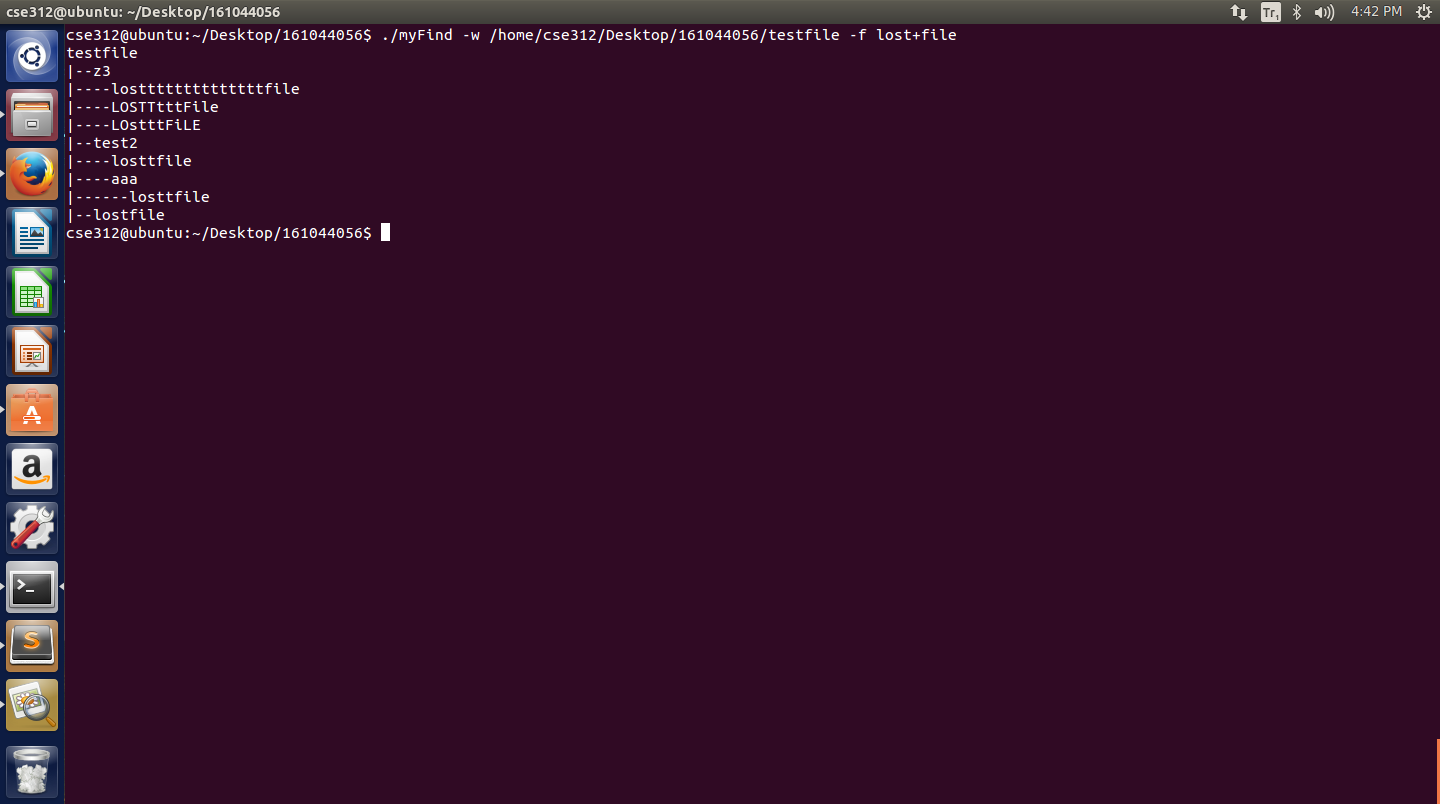
\includegraphics[scale=0.3]{example-run1.png}
\caption{Example with full path}
\label{fig:example-run1.png}
\end{figure}

Also,if directory in same folder as code user can just give filename like
-w testfile
\begin{figure}[h!]
\centering
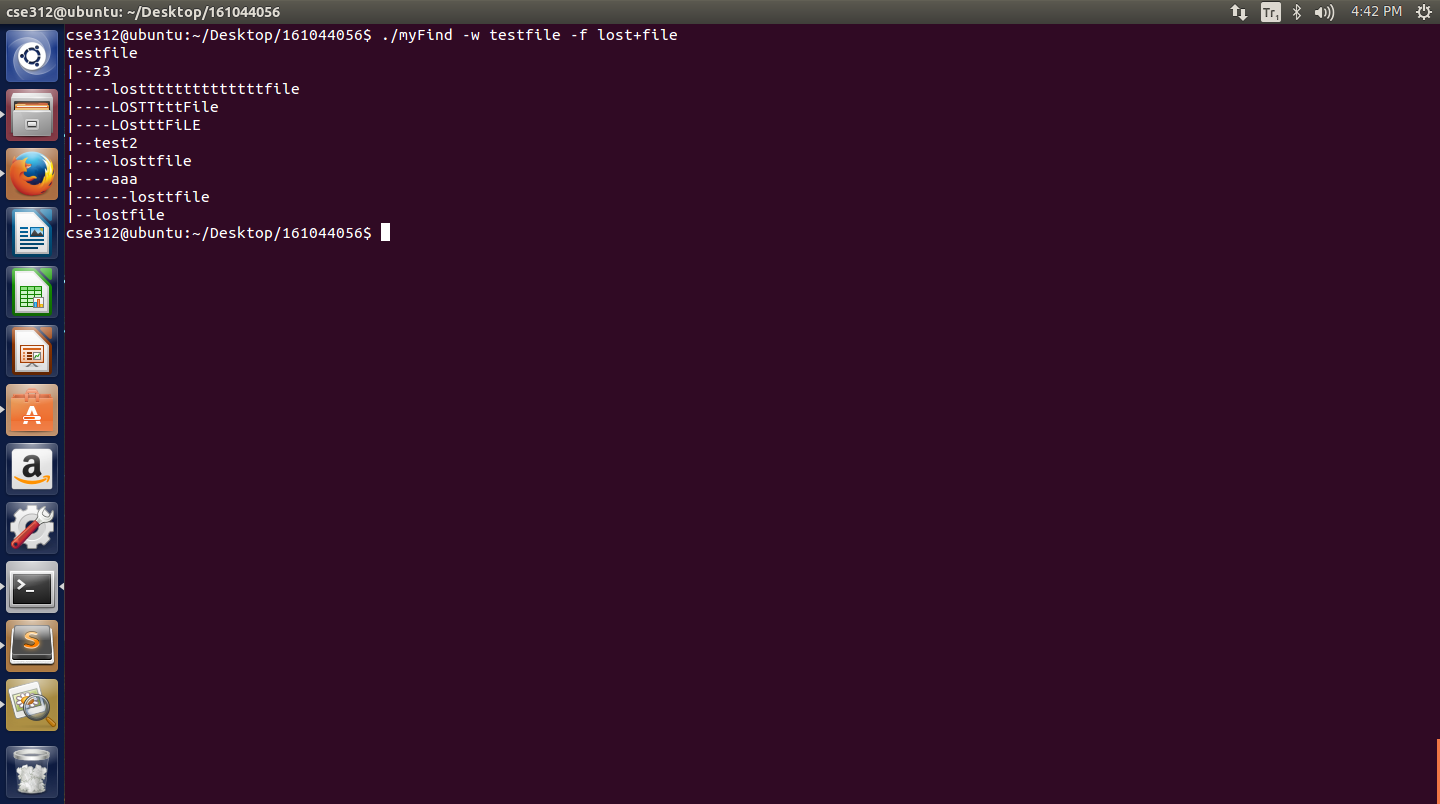
\includegraphics[scale=0.3]{example-run2.png}
\caption{Example with filename}
\label{fig:example-run1.png}
\end{figure}


\begin{figure}[h!]
\centering
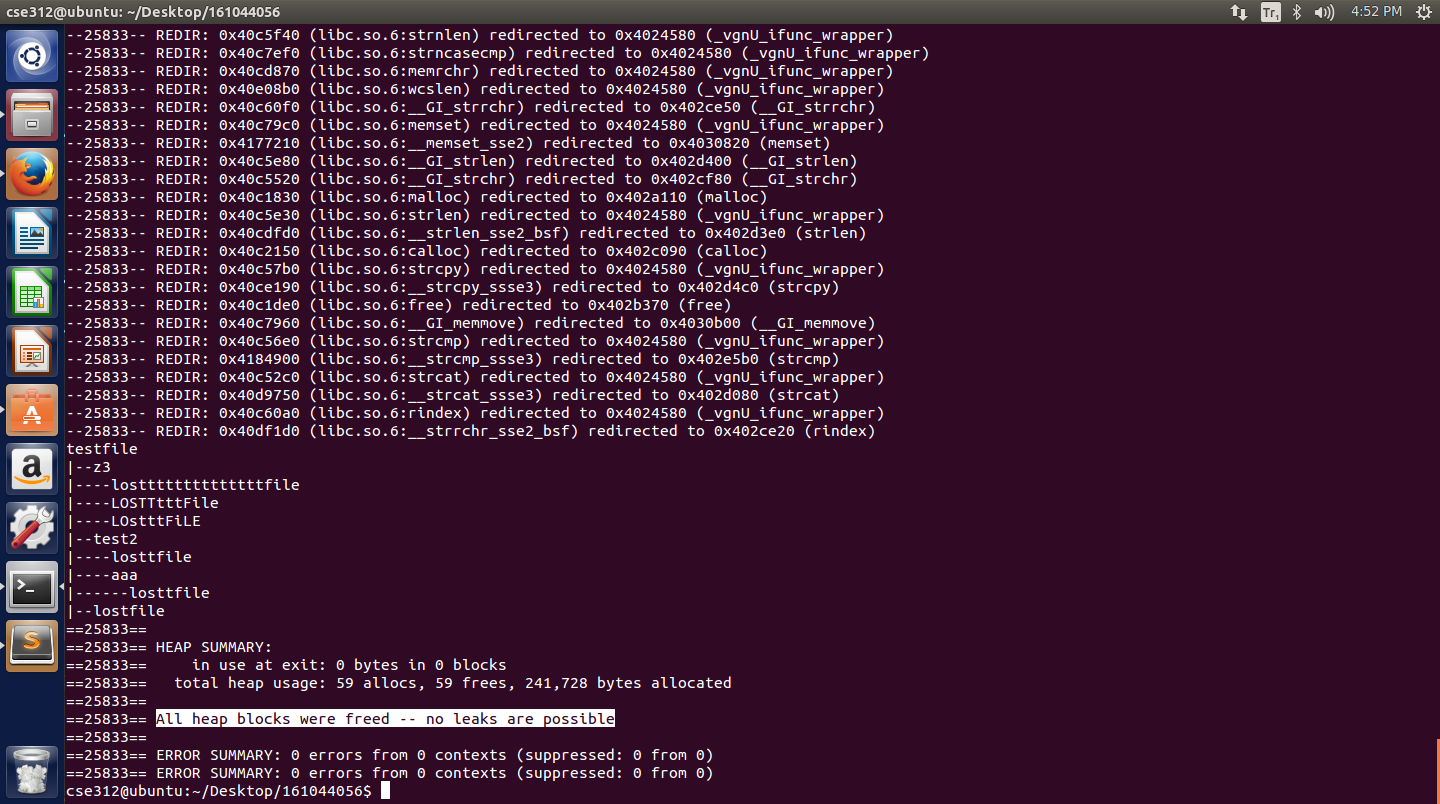
\includegraphics[scale=0.3]{example-run3.png}
\caption{Example with Valgrind}
\label{fig:example-run3.png}
\end{figure}

As you can see there is no leak when execute program with valgrind


\end{document}
